%!TEX TS-program = xelatex
%!TEX options = -aux-directory=Debug -shell-escape -file-line-error -interaction=nonstopmode -halt-on-error -synctex=1 "%DOC%"
\documentclass{article}
\input{LaTeX-Submodule/template.tex}

% Additional packages & macros
\usepackage{changepage} % Modify page width
\usepackage{multicol} % Use multiple columns
\usepackage[explicit]{titlesec} % Modify section heading styles
\setitemize{leftmargin=*,topsep=1ex,partopsep=0ex,itemsep=-1ex,partopsep=0ex,parsep=1ex}
\setlist{leftmargin=*,topsep=1ex,partopsep=0ex,itemsep=-1ex,partopsep=0ex,parsep=1ex}

\titleformat{\section}{\raggedright\normalfont\bfseries}{}{0em}{#1}
\titleformat{\subsection}{\raggedright\normalfont\small\bfseries}{}{0em}{#1}
\titleformat{\subsubsection}{\raggedright\normalfont\small\bfseries}{}{0em}{#1}

%% A4 page
\geometry{
	a4paper,
	margin = 10mm
}

%% Hide horizontal rule
\renewcommand{\headrulewidth}{0pt}
\fancyhead{}

%% Hide page numbers
\pagenumbering{gobble}

%% Multi-columns setup
\setlength\columnsep{4pt}

%% Paragraph setup
\setlength\parindent{0pt}
\setlength\parskip{0pt}

\begin{document}
% Modify spacing
\titlespacing*\section{0pt}{1ex}{1ex}
\titlespacing*\subsection{0pt}{1ex}{1ex}
%
\setlength\abovecaptionskip{8pt}
\setlength\belowcaptionskip{-15pt}
\setlength\textfloatsep{0pt}
%
\setlength\abovedisplayskip{1pt}
\setlength\belowdisplayskip{1pt}
\begin{multicols*}{3}
    \section{Fourier Series}
    Approximate \(f\) on \(\interval{-L}{L}\) by
    \begin{multline*}
        f_F\left( x \right) = a_0 + \\
        \sum_{n = 1}^\infty \left[ a_n \cos{\left( \omega_n x \right)} + b_n \sin{\left( \omega_n x \right)} \right]
    \end{multline*}
    where \(\omega_n = \frac{n \pi}{L}\) and
    \(f = f_F\) on \(\interval{-L}{L}\) and \textbf{periodically extended} elsewhere.
    \begin{align*}
        a_0 & = \frac{1}{2L} \int_{-L}^L f\left( x \right) \odif{x}                                \\
        a_n & = \frac{1}{L} \int_{-L}^L f\left( x \right) \cos{\left( \omega_n x \right)} \odif{x} \\
        b_n & = \frac{1}{L} \int_{-L}^L f\left( x \right) \sin{\left( \omega_n x \right)} \odif{x}
    \end{align*}
    for \(n \in \N\).
    \subsection{Integral Relationships}
    \begin{align*}
        \int_{-L}^L \cos{\left( \omega_n x \right)} \odif{x}                                 & = 0 \\
        \int_{-L}^L \sin{\left( \omega_n x \right)} \odif{x}                                 & = 0 \\
        \int_{-L}^L \sin{\left( \omega_n x \right)} \cos{\left( \omega_m x \right)} \odif{x} & = 0
    \end{align*}
    for \(n, m \in \N\)
    \begin{align*}
        \int_{-L}^L \cos{\left( \omega_n x \right)} \cos{\left( \omega_m x \right)} \odif{x} & = L \\
        \int_{-L}^L \sin{\left( \omega_n x \right)} \sin{\left( \omega_m x \right)} \odif{x} & = L
    \end{align*}
    when \(n = m\), and \(0\) otherwise.
    \subsection{Cosine (Even) Series}
    When \(f\) is even, \(b_n = 0\), and
    \begin{align*}
        a_0 & = \frac{1}{L} \int_0^L f\left( x \right) \odif{x}                                 \\
        a_n & = \frac{2}{L} \int_0^L f\left( x \right) \cos{\left( \omega_n x \right)} \odif{x}
    \end{align*}
    \subsection{Sine (Odd) Series}
    When \(f\) is odd, \(a_0 = a_n = 0\), and
    \begin{equation*}
        b_n = \frac{2}{L} \int_0^L f\left( x \right) \sin{\left( \omega_n x \right)} \odif{x}
    \end{equation*}
    Both expansions result in even/odd periodic extensions of \(f\).
    \section{Partial Differential Equations}
    \begin{itemize}
        \item \textbf{Dirichlet} \(u\left( a,\: t \right) = C\)
        \item \textbf{Neumann} \(\pdv{u}{x} \left( a,\: t \right) = C\)
        \item \textbf{Robin} \(A u\left( a,\: t \right) + B \pdv{u}{x} \left( a,\: t \right) = C\)
    \end{itemize}
    \subsection{Separation of Variables}
    \begin{equation*}
        u_n\left( x,\: t \right) = X_n\left( x \right) T_n\left( t \right)
    \end{equation*}
    on some finite interval \(\interval{a}{b}\) with \(t \geqslant 0\).
    Substitute and separate into two ODEs:
    \begin{align*}
        f_1\left( x,\: X,\: X',\: \dots \right) & = \alpha_n \\
        f_2\left( t,\: T,\: T',\: \dots \right) & = \alpha_n
    \end{align*}
    Solve ODE with BCs to find eigenvalues \(\alpha_n\) and eigenfunctions \(X_n\).
    Solve other ODE to find \(u_n\left( t \right)\).
    Apply superposition and solve ICs to find \(u\left( x,\: t \right)\).

    Given two spatial dimensions, consider the ODE with
    homogeneous BCs first.
    \subsection{Polar Coordinates}
    \begin{equation*}
        u\left( r,\: \theta \right) = R\left( r \right) \Theta\left( \theta \right)
    \end{equation*}
    with periodicity:
    \(\Theta\left( \theta \right) = \Theta\left( \theta + 2 \pi \right)\).

    For radially symmetric problems
    \begin{equation*}
        u\left( r,\: t \right) = R\left( r \right) T\left( t \right)
    \end{equation*}
    with \(\pdv{u}{\theta} = 0\).

    Solutions require \textbf{boundedness} in \(r\).
    \section{Sturm-Liouville Theory}
    \begin{equation*}
        \odv{}{x} \left[ p\left( x \right) \odv{y}{x} \right] + q\left( x \right) y + \lambda w\left( x \right) y = 0
    \end{equation*}
    with two non-trivial homogeneous BCs:
    \begin{align*}
        -l_1 y'\left( a \right) + h_1 y\left( a \right) & = 0 \\
        l_2 y'\left( b \right) + h_2 y\left( b \right)  & = 0
    \end{align*}
    have infinitely many \(\lambda_n\) and \(y_n\),
    where \(\lambda_n \to \infty \) as \(n \to \infty\).
    \(\left\{ y_n : n \in \Z^{+} \right\}\) form an orthogonal basis that satisfy the BCs.
    \begin{equation*}
        y \mapsto - \frac{1}{w\left( x \right)} \left( \odv{}{x} \left[ p\left( x \right) \odv{y}{x} \right] + q\left( x \right) y \right)
    \end{equation*}
    \begin{itemize}
        \item \textbf{Regular} when \(p, w > 0\), and \(p, p', q, w\) are continuous
              over the interval \(\interval{a}{b}\).
        \item \textbf{Proper} when \(q\left( x \right) \leqslant 0\) on \(\interval{a}{b}\),
              with \(l_1h_1 \geqslant 0\) and \(l_2h_2 \geqslant 0\).
              All eigenvalues are non-negative.
        \item \textbf{Singular} when \(p\left( a \right) = 0\), and \(x = a\) is replaced by the condition that
              \(y\) remain bounded.
        \item \textbf{Periodic} when instead of BCs we have, \(p\left( a \right) = p\left( b \right)\) and \(p'\left( a \right) = p'\left( b \right)\).
              \(y\) is then also periodic.
    \end{itemize}
    Transform the ODE
    \begin{equation*}
        a_2 y'' + a_1 y' + a_0 y = \lambda y
    \end{equation*}
    with the integrating factor:
    \begin{equation*}
        \mu = \frac{1}{a_2} \exp{\left( \int \frac{a_1}{a_2} \odif{x} \right)}.
    \end{equation*}
    \subsection{Weighted Inner-Product}
    \begin{equation*}
        \abracket*{y_n,\: y_m} = \int_a^b y_n y_m w \odif{x} = \delta_{mn}
    \end{equation*}
    \subsubsection{Eigenfunction Expansion}
    Approximate \(f\) on \(\interval{a}{b}\) by
    \begin{equation*}
        f_E = \sum_{n = 1}^\infty c_n y_n = \sum_{n = 1}^\infty \frac{\abracket*{f,\: y_n}_w}{\abracket*{y_n,\: y_n}_w} y_n.
    \end{equation*}
    where \(c_m\) is found via the inner-product:
    \begin{equation*}
        \abracket*{f,\: y_m}_w = \sum_{n = 1}^\infty c_n \abracket*{y_n,\: y_m}_w
    \end{equation*}
    \section{Nonhomogeneous Problems}
    For time-dependent problems, separate solution into \textbf{steady-state} part
    \begin{equation*}
        U\left( x \right)
    \end{equation*}
    which is found by setting \(u_t = 0\), and \textbf{transient} part
    \begin{equation*}
        v\left( x,\: t \right) = u\left( x, \: t \right) - U\left( x \right)
    \end{equation*}
    and solve via substitution.
    \subsection{Eigenfunction Expansion}
    Assume the solution takes the form of an eigenfunction expansion in
    one variable. Here the boundary conditions must be homogeneous.
    \section{Integral Transforms}
    \subsection{Fourier Transform \texorpdfstring{\(\mathscr{F}\)}{F}}
    \begin{align*}
        \hat{f}\left( \omega \right) & = \int_{-\infty}^\infty f\left( x \right) e^{-i \omega x} \odif{x}                               \\
        f_F\left( x \right)          & = \frac{1}{2\pi} \int_{-\infty}^\infty \hat{f}\left( \omega \right) e^{i \omega x} \odif{\omega}
    \end{align*}
    Solve PDEs on infinite domains where \(u\) is bounded at \(\pm \infty\).
    \subsubsection{Convolution Theorem}
    \begin{equation*}
        \left( f \ast g \right)\left( x \right) = \int_{-\infty}^\infty f\left( x - z \right) g\left( z \right) \odif{z}
    \end{equation*}
    \begin{align*}
        \mathscr{F}\left\{ f g \right\}                  & = \frac{1}{2\pi} \left( \hat{f} \ast \hat{g} \right)\left( \omega \right) \\
        \mathscr{F}^{-1}\left\{ \hat{f} \hat{g} \right\} & = \left( f \ast g \right)\left( x \right)
    \end{align*}
    \subsection{Laplace Transform \texorpdfstring{\(\mathscr{L}\)}{L}}
    \begin{align*}
        F\left( s \right) & = \int_0^\infty f\left( t \right) e^{-st} \odif{t}                                                \\
        f\left( t \right) & = \frac{1}{2\pi i} \int_{\sigma - i \infty}^{\sigma + i \infty} F\left( s \right) e^{st} \odif{s}
    \end{align*}
    for sufficiently large \(\sigma\) so that \(f\left( t \right) e^{\sigma t} \to 0\) as \(t \to \infty\). \(\sigma\) must be to the right of all singularities.
    \subsubsection{Convolution Theorem}
    \begin{equation*}
        \left( f \ast g \right)\left( t \right) = \int_0^t f\left( t - \tau \right) g\left( \tau \right) \odif{\tau}
    \end{equation*}
    \begin{align*}
        \mathscr{L}\left\{ f g \right\}      & = \left( F \ast G \right)\left( s \right) \\
        \mathscr{L}^{-1}\left\{ F G \right\} & = \left( f \ast g \right)\left( t \right)
    \end{align*}
    \section{Specific PDE Problems}
    \subsection{Heat Equation}
    \begin{equation*}
        \pdv{u}{t} = k \pdv[order=2]{u}{x}
    \end{equation*}
    \subsection{Wave Equation}
    \begin{equation*}
        \pdv[order=2]{u}{t} = c^2 \pdv[order=2]{u}{x}
    \end{equation*}
    \subsection{Laplace's Equation}
    \begin{equation*}
        \nabla^2 u = \pdv[order=2]{u}{x} + \pdv[order=2]{u}{y} = 0
    \end{equation*}
    \section{Common Taylor Series}
    \begin{align*}
        e^z                     & = \sum_{n = 0}^\infty \frac{z^n}{n!}, \abs*{z} < \infty                                                \\
        \cos{\left( z \right)}  & = \sum_{n = 0}^\infty \frac{\left( -1 \right)^n z^{2n}}{\left( 2n \right)!}, \abs*{z} < \infty         \\
        \sin{\left( z \right)}  & = \sum_{n = 0}^\infty \frac{\left( -1 \right)^n z^{2n + 1}}{\left( 2n + 1 \right)!}, \abs*{z} < \infty \\
        \cosh{\left( z \right)} & = \sum_{n = 0}^\infty \frac{z^{2n}}{\left( 2n \right)!}, \abs*{z} < \infty                             \\
        \sinh{\left( z \right)} & = \sum_{n = 0}^\infty \frac{z^{2n + 1}}{\left( 2n + 1 \right)!}, \abs*{z} < \infty                     \\
        \frac{1}{1 - z}         & = \sum_{n = 0}^\infty z^n, \abs*{z} < 1
    \end{align*}
\end{multicols*}
\begin{multicols*}{3}
    \section{Complex Analysis}
    \subsection{Complex-Valued Functions}
    \begin{equation*}
        w = f\left( z \right) = u\left( x, \: y \right) + i v\left( x, \: y \right)
    \end{equation*}
    where \(w = u + iv\) and \(z = x + iy\).
    \subsection{Analytic Functions}
    \(f\) satisfies \textbf{Cauchy-Riemann} equations:
    \begin{equation*}
        \pdv{u}{x} = \pdv{v}{y}, \quad \pdv{v}{x} = -\pdv{u}{y}.
    \end{equation*}
    The derivative is given by
    \begin{equation*}
        \odv{f}{z} = \pdv{u}{x} + i \pdv{v}{x} = \pdv{v}{y} - i \pdv{u}{y}.
    \end{equation*}
    As \(z\) is a complex number, the limit
    \begin{equation*}
        \lim_{z \to z_0} f\left( z \right) = L
    \end{equation*}
    must be path independent.
    If a function is differentiable at a point and in its neighbourhood,
    it is analytic at that point.
    Analytic functions are infinitely differentiable and
    have convergent Taylor series expansions near that point.
    \subsection{Complex Differentiation}
    Polynomials, rational functions (except at singularities), and exponentials
    follow familiar rules. As do any sums, products, or compositions of these functions.

    Logarithms, non-integer powers, and inverse trigonometric functions behave similarly,
    except at branch points and branch cuts.
    \subsection{Laplace's Equation}
    If \(f\) is analytic in a region \(\mathcal{D}\),
    then \(u\) and \(v\) both satisfy Laplace's equations
    \(\nabla^2 u = 0\), \(\nabla^2 v = 0\)
    in \(\mathcal{D}\). \(u\) and \(v\) are \textbf{harmonic} functions
    and \(v\) is the \textbf{harmonic conjugate} of \(u\).
    \subsection{Complex Integration}
    Compute line integrals in the complex plane,
    where an oriented curve \(C\) is parametrised by
    \begin{equation*}
        z\left( t \right) = x\left( t \right) + i y\left( t \right)
    \end{equation*}
    for \(t \in \interval{a}{b}\). A curve is:
    \begin{itemize}
        \item \textbf{Smooth} if \(\pdv{z}{t}\) is piecewise continuous and nonzero for all \(t\).
        \item \textbf{Closed} if \(z\left( a \right) = z\left( b \right)\).
        \item \textbf{Simple} if it does not cross itself: \(z\left( t_1 \right) \neq z\left( t_2 \right)\) for \(t_1 \neq t_2\), \(a < t_1\), \(t_2 < b\).
    \end{itemize}
    \subsection{Complex Line Integrals}
    \begin{equation*}
        \int_C f\left( z \right) \odif{z} = \int_a^b f\left( z\left( t \right) \right) \odv{z}{t} \odif{t}
    \end{equation*}
    \subsection{Cauchy's Integral Theorem}
    If \(f\) is analytic in a region \(\mathcal{D}\), then
    the contour integral along any simple closed curve \(C\) in \(\mathcal{D}\) is zero
    \begin{equation*}
        \oint_C f\left( z \right) \odif{z} = 0.
    \end{equation*}
    For any two points \(z_1, z_2 \in \mathcal{D}\),
    \begin{equation*}
        \int_{C_1} f\left( z \right) \odif{z} = \int_{C_2} f\left( z \right) \odif{z}
    \end{equation*}
    where \(C_1\) and \(C_2\) are any two paths from \(z_1\) to \(z_2\).
    This is because the integral along the closed curve \(C_1 - C_2\) is zero by CIT.

    The same holds for an annulus where two simple closed curves \(C_1\) and \(C_2\)
    have nonzero integrals, but the integral along \(C_1 + C_3 - C_2 + C_4\) is zero,
    where \(C_3 = -C_4\) are paths connecting \(C_1\) and \(C_2\).
    \subsection{Cauchy's Integral Formula}
    If \(f\) is analytic on and within a simple closed curve \(C\),
    then for any point \(z_0\) within \(C\)
    \begin{equation*}
        f\left( z_0 \right) = \frac{1}{2 \pi i} \oint_C \frac{f\left( z \right)}{z - z_0} \odif{z}
    \end{equation*}
    \subsection{Isolated Singularities}
    Suppose \(f\) is analytic in \(V = U\backslash\left\{ z_0 \right\}\), then \(z_0\) is a \textbf{singularity} of \(f\).
    Assume the existence of \(g\) such that \(g\) is analytic in \(U\). Then the singularity of \(f\) at \(z_0\) is:
    \begin{itemize}
        \item \textbf{Removable} (no negative powers)
              \begin{equation*}
                  \forall z \in U,\: \exists g : f\left( z \right) = g\left( z \right)
              \end{equation*}
        \item \textbf{Pole} (finitely many negative powers)
              \begin{equation*}
                  \forall z \in V : \exists g : g\left( z \right) = \left( z - z_0 \right)^n f\left( z \right)
              \end{equation*}
              where \(g\left( z_0 \right) \neq 0\).
              The \textbf{order} of a pole is the largest value of \(n\)
              (smallest power in Laurent series). When \(n = 1\), \(z_0\) is a \textbf{simple pole}.
        \item \textbf{Essential} (infinitely many negative powers)
    \end{itemize}
    \subsection{Laurent Series Expansion}
    If \(f\) is analytic on \(0 < \abs{z - z_0} < d\), but contains
    an \textbf{isolated singularity} at \(z_0\), then \(f\) can be
    represented by
    \begin{equation*}
        f\left( z \right) = \sum_{n = -\infty}^\infty a_n \left( z - z_0 \right)^n
    \end{equation*}
    where \(a_n \in \C\).
    \subsection{Residues (\texorpdfstring{\(a_{-1}\)}{a-1} term)}
    For a simple pole,
    \begin{equation*}
        \Res_{z = z_0} f\left( z \right) = \lim_{z \to z_0} \left( z - z_0 \right) f\left( z \right).
    \end{equation*}
    For a pole of order \(n\),
    \begin{multline*}
        \Res_{z = z_0} f\left( z \right) = \frac{1}{\left( n - 1 \right)!} \\
        \lim_{z \to z_0} \odv[order={n - 1}]{}{z} \biggl[ \left( z - z_0 \right)^n f\left( z \right) \biggr].
    \end{multline*}
    \subsection{Residue Theorem}
    If \(f\) be analytic on and within a simple closed curve \(C\),
    except for a finite number of isolated singularities \(z_1, \ldots, z_n \in C\)
    \begin{equation*}
        \oint_C f\left( z \right) \odif{z} = 2 \pi i \sum_{k = 1}^n \Res_{z = z_k} f\left( z \right).
    \end{equation*}
    \subsection{Jordan's Lemma}
    Consider a large semi-circular curve \(C_R\) centred at \(s = \sigma\), extending toward the left hand plane:
    \(s\left( \theta \right) = \sigma + R e^{i \theta}\) with \(\pi/2 < \theta < 3\pi/2\).
    If \(F\left( s \right) \to 0\) as \(\abs*{s} \to \infty\) for all \(s\) on \(C_R\),
    then
    \begin{equation*}
        \lim_{R \to \infty} \int_{C_R} F\left( s \right) e^{s t} \odif{s} = 0.
    \end{equation*}
    Adding this integral to the inverse Laplace transform integral
    creates a closed curve, so by the residue theorem
    \begin{equation*}
        f\left( t \right) = \sum_{k = 1}^n \Res_{s = s_k} F\left( s \right) e^{s t}
    \end{equation*}
    \subsection{Fourier Transform}
    Integrating in the complex \(x\)/\(\omega\) plane, along the real axis, consider a semi-circle in the upper/lower half plane,
    where the direction depends on the sign of \(\omega\)/\(x\).
    \begin{itemize}
        \item \textbf{Forward} (\(e^{-i\omega x}\)), \(\omega \in \R\), \(x \in \C\):
        \begin{itemize}
            \item If \(\omega < 0\), \(\abs*{e^{-i \omega x}} = e^{\omega \Im{\left( x \right)}} \to 0\) as \(\Im{\left( x \right)} \to \infty\).
            (upper half \(x\)-plane).
            \item If \(\omega > 0\), \(\abs*{e^{-i \omega x}} = e^{\omega \Im{\left( x \right)}} \to 0\) as \(\Im{\left( x \right)} \to -\infty\).
            (lower half \(x\)-plane).
        \end{itemize}
        \item \textbf{Inverse} (\(e^{i\omega x}\)), \(\omega \in \C\), \(x \in \R\):
        \begin{itemize}
            \item If \(x < 0\), \(\abs*{e^{i \omega x}} = e^{-x \Im{\left( \omega \right)}} \to 0\) as \(\Im{\left( \omega \right)} \to -\infty\).
            (lower half \(\omega\)-plane).
            \item If \(x > 0\), \(\abs*{e^{i \omega x}} = e^{-x \Im{\left( \omega \right)}} \to 0\) as \(\Im{\left( \omega \right)} \to \infty\).
            (upper half \(\omega\)-plane).
        \end{itemize}
    \end{itemize}
    \subsection{Useful Results}
    \begin{equation*}
        \oint_C z^n \odif{z} = \int_0^{2\pi} \left( Re^{it} \right)^n iRe^{it} \odif{t} = 2\pi i
    \end{equation*}
    when \(n = -1\), and \(0\) otherwise, for a circle of radius \(R\) oriented anti-clockwise.
    \subsection{Hyperbolic Functions}
    \begin{align*}
        \cos{\left( z \right)}    & = \frac{e^{iz} + e^{-iz}}{2}  \\
        \sin{\left( z \right)}    & = \frac{e^{iz} - e^{-iz}}{2i} \\
        \cosh{\left( z \right)}   & = \frac{e^z + e^{-z}}{2}      \\
        \sinh{\left( z \right)}   & = \frac{e^z - e^{-z}}{2}      \\
        \cosh{\left( i z \right)} & = \cos{\left( z \right)}      \\
        \sinh{\left( i z \right)} & = i \sin{\left( z \right)}
    \end{align*}
    \(\sinh{\left( z \right)} = 0\) when \(z = n \pi i\) for \(n \in \Z\).
    \(\cosh{\left( z \right)} = 0\) when \(z = n \pi i + \pi i / 2\) for \(n \in \Z\).
    \begin{figure}[H]
        \centering
        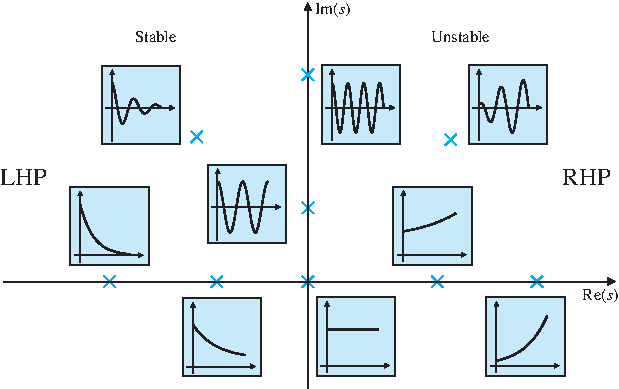
\includegraphics[width=\linewidth,angle=90]{Figures/stabilitysplane.pdf}
    \end{figure}
\end{multicols*}
\end{document}
